%===============================================================================
%------ Preambulo---------------------------------------------------------------
%===============================================================================
% arara: pdflatex: { synctex: on, shell: yes }
% arara: bibtex
% arara: pdflatex: { synctex: on, shell: yes }
% arara: pdflatex: { synctex: on, shell: yes }
%-------------------------------------------------------------------------------
\documentclass[ %
	Journal, %
	FontSize=10pt
]{../Preamble/UMSAetn}

\usepackage[ %
	University={Universidad Mayor de San Andrés}, %
	UniversityWeb={http://umsa.edu.bo}, %
	Faculty={Facultad de Ingeniería}, %
	FacultyWeb={http://miing.umsa.edu.bo}, %
	Department={Carrera de Ingeniería Electrónica}, %
	DepartmentWeb={http://miing.umsa.edu.bo}, %
	Group={Instituto de Electrónica Aplicada - IEA}, %
	GroupWeb={http://miing.umsa.edu.bo}, %
	%
	Title={Título Journal}, %
	Subtitle={Subtitulo}, %
	Editor={Paulo Roberto Loma Marconi}, %
	EditorEmail={mailto:prlomarconi@gmail.com}, %
	Header={Journal - IEA}, %
	%
	FiguresPath={Figures/}, %	
	BibPath={BibliographyJournal.bib}
]{../Preamble/Administrative}

%-------------------------------------------------------------------------------
\begin{document}
	%---- Paginas delanteras ---------------------------------------------------
	%------------------------------------------------------------------------------------
%	Titulo propio
%------------------------------------------------------------------------------------
\begin{titlepage}
	\begin{center}		
		\textsc{\LARGE {\myUniversity}}\\[0.5cm] 
		\textsc{\Large{\myFaculty}}\\[0.5cm]
		\textsc{\large{\myDepartment}}\\[1cm]	
		
\includegraphics[width=0.12\linewidth]{logoumsa}\\[1cm] 		
		\textsc{\LARGE Perfil de Proyecto de Grado}\\[1.5cm]
		\textsc{\Large \myTitle}\\[2cm]									
		\begin{minipage}{0.8\textwidth}
			\begin{flushleft} 
				\large\textit{Autor:}\quad\myAuthorName\\[0.5cm]
				\large\textit{Asesor:}\quad\myAsesorName\\[0.5cm]
				\large\textit{DAM:}\quad\ \mySupervisorName\\[0.5cm]
			\end{flushleft}
		\end{minipage}\\[2cm]	
		\today	
		\vfill
	\end{center}	
\end{titlepage}	
	\tableofcontents
	\chapter{intro}
	\section{seccion 1}
	artículo  pág. \pageref{art1}, articulo según toc \ref{art1}
	%---- Contenido principal --------------------------------------------------	
	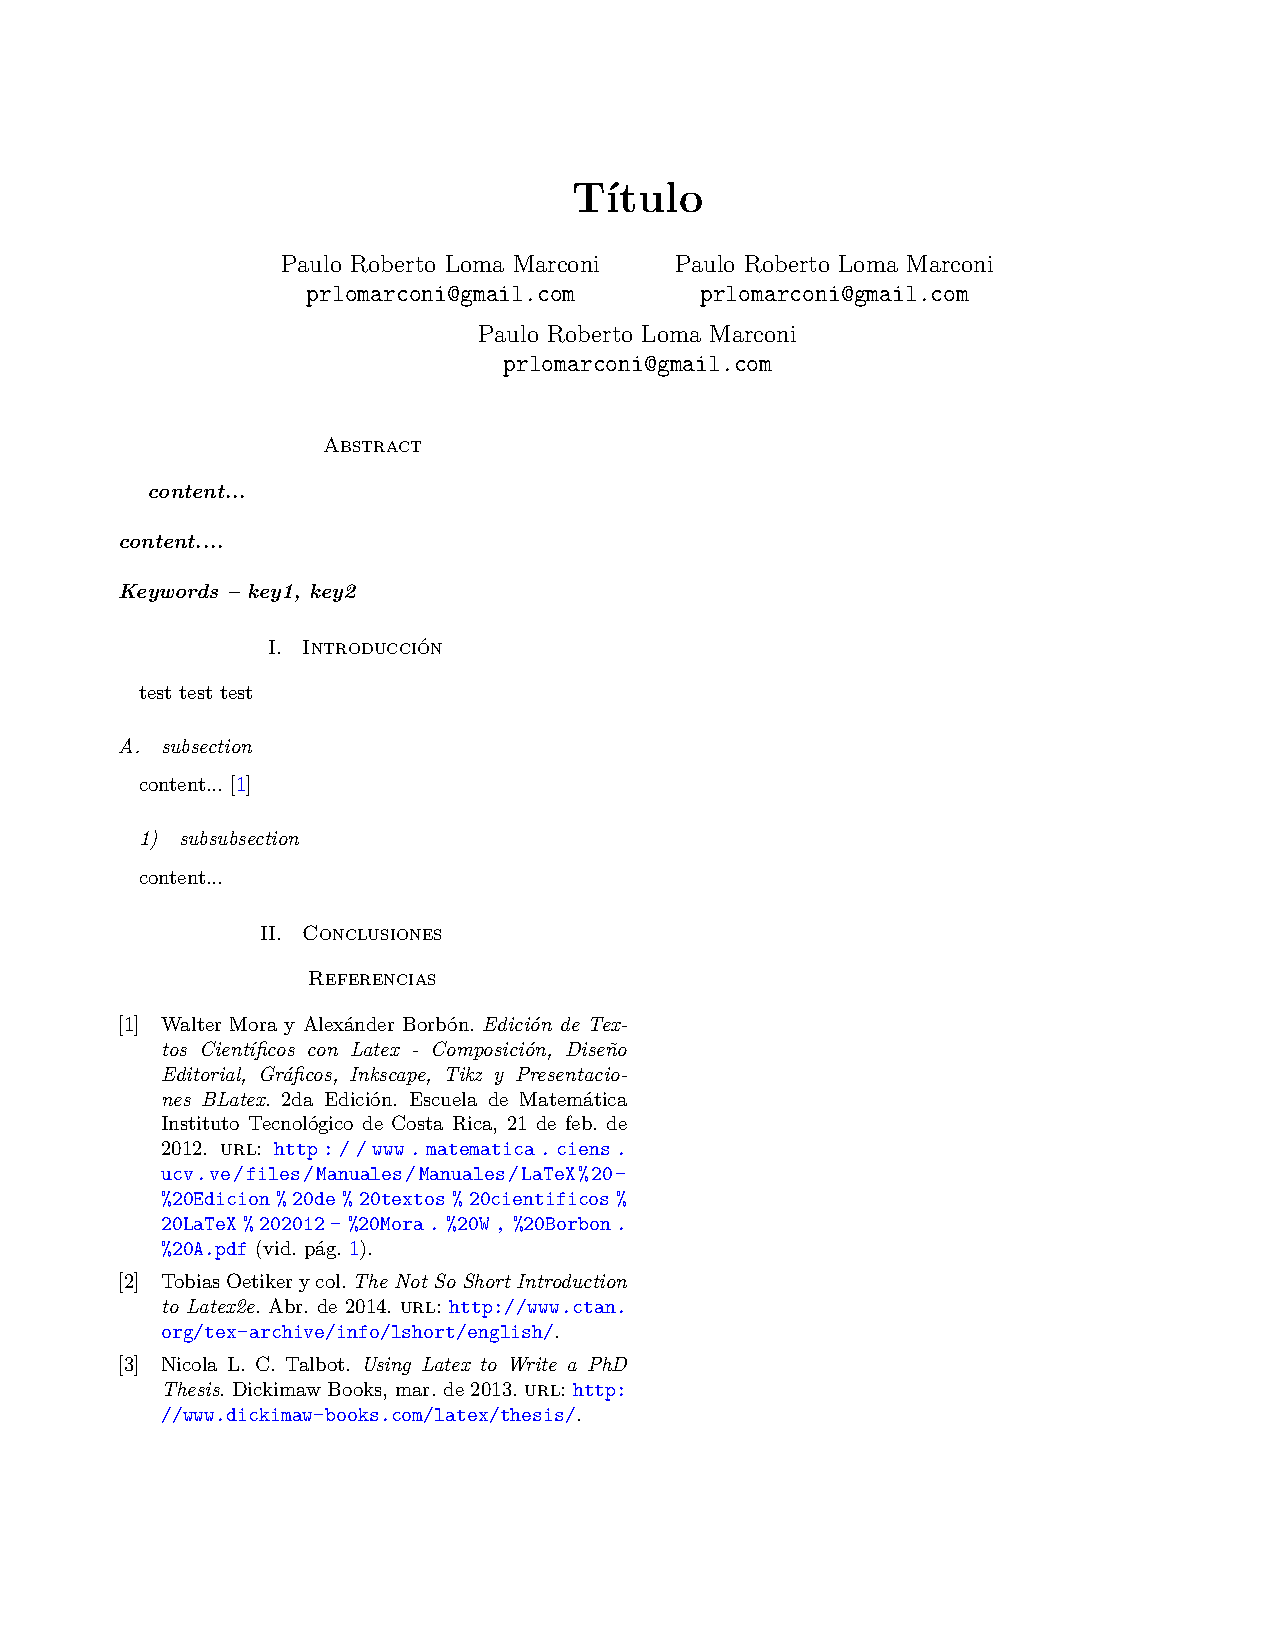
\includepdf[pages=1-,pagecommand={\thispagestyle{fancy}}, %
		addtotoc={1, %page number
			chapter, %section
			1, %level
			{Título de un Artículo.}, %title
			art1 %label
		} 
	]{../ArticlesIEA/Article1/Article1.pdf}
	%---- Paginas finales ------------------------------------------------------	
	\printbibliography
	\addcontentsline{toc}{chapter}{\bibname}
	\nocite{*} % imprime todo el contenido de la bibliografía aunque no este citado 	    
\end{document}